% Conference version (single column, 9 pages of main text) of paper/main_en.tex, the full version (arXiv/journal).
% Written 2026-10-21 by condensing the full version; it adds no numbers or claims of its own
% (check: scripts/2026-10-21/check_short_numbers.py). Tables and figures are \input from floats_en/,
% generated from main_en.tex by scripts/2026-10-21/extract_floats.py, so they stay identical to the full version.
% Page budget mimics a typical single-column venue: letter paper, 5.5 x 9 in text area, 10 pt Times-like font.
% Compile with XeLaTeX.
\documentclass[10pt]{article}
\usepackage[letterpaper,textwidth=5.5in,textheight=9in,top=1in,headsep=0.25in]{geometry}
\usepackage{fontspec}
\IfFontExistsTF{TeX Gyre Termes}{\setmainfont{TeX Gyre Termes}}{}
\usepackage{amsmath,amssymb}
\usepackage{graphicx}
\usepackage{booktabs,tabularx,array,multirow}
\usepackage[numbers,sort&compress]{natbib}
\usepackage{enumitem}
\usepackage{caption}
\usepackage[section]{placeins}
\usepackage{xcolor}
\usepackage{xurl}
\usepackage[hidelinks]{hyperref}
\captionsetup{font=small,labelfont=bf}
\graphicspath{{figures/}}
\newcolumntype{L}{>{\raggedright\arraybackslash}X}
\newcommand{\code}[1]{\texttt{#1}}
\setlist{itemsep=1pt,topsep=3pt}
\setlength{\emergencystretch}{3em}

\title{Failure Prediction in Small Qwen Language-Model Agents:\\Hidden-State Probes Do Not Beat Visible Information}
\author{Author information withheld for review}
\date{}

\begin{document}
\maketitle

\begin{abstract}
Linear probes on the hidden states of language-model agents have been proposed as cheap monitors that predict failure early, but their gains have been measured against baselines that do not see the task.
We tested whether such probes predict failure beyond the information visible in the prompt for a 3-billion-parameter Qwen2.5 agent in the ALFWorld household text environment,
between games (500 greedy episodes) and within games (100 games run eight times each), against a ladder of baselines built from the task type, the prompt text and progress features, with all data split by room layout and the primary analysis fixed before it was run once.
In the pre-registered comparison (probe at 50\% depth) the probe was below the full baseline at the first three actions by 0.13 to 0.18 in AUROC (all 95\% confidence intervals below zero; the second action only narrowly after a rough correction for interval coverage), and on 250 held-out games no action was superior.
Within games, the probe and the baselines all separated failed from successful attempts above chance from the third action, but the probe was superior in none of six comparisons.
With a four-billion-parameter Qwen3 agent and with an external prompt the probe was again superior at no action, and under the external prompt it was below the baseline at the third action.
Used to stop failing episodes with at most 10\% of successes lost, the probe was not shown to save more actions than a fixed limit.
We found no gain from hidden states; for the one configuration tested on held-out games (75\% depth) the single hold-out's intervals exclude gains above about 0.10 AUROC, but smaller gains cannot be ruled out.
Claims of hidden-state failure signals in agents should be tested against baselines that see the task, and within tasks.
\end{abstract}

\section{Introduction}
An agent episode that ends in failure consumes as much computation as one that succeeds, and the cost matters most where agents run locally~\cite{pham2026agentstop}.
In our setting, a Qwen2.5-3B agent solved 22.4\% of the first 250 ALFWorld games, and failed episodes accounted for 89.7\% of the executed steps.
Stopping doomed episodes early could recover much of this cost, but for a small agent the monitor itself must be cheap: a 0.6B text monitor adds only 0.1--0.6\% compute to 9--31B policies~\cite{wang2026failfast},
and is 15--52 times cheaper per token than those policies, whereas a separate 0.5B monitor that reads every token a 3B actor reads would add about 13--16\% of the actor's compute. A probe on the hidden states the actor already computes needs no additional model call.

Ruan et al.~\cite{ruan2026doomed} reported that such a probe predicts the eventual failure of multi-step agents from the first rounds and is consistently stronger than a scorer built from behavioral features.
These reports leave one question open: does the signal show how the current attempt is going, or which task the agent faces?
Outcomes are largely determined by the task: in our sampled data, whose games were stratified by greedy outcome, the game explains 69.5\% of the outcome variance, and in repeated HotpotQA runs 64 of 100 questions were answered correctly in every run and 23 in none~\cite{mehta2026commit}.
A pooled AUROC is a weighted sum of a within-task and a between-task component, and a predictor that depends on the task alone scores exactly 0.5 within a task~\cite{bulut2026problem}.
Moreover, the comparison baselines in agent studies have been weak: the behavioral scorer of~\cite{ruan2026doomed} sees neither the task statement nor the observations, whereas in our data the task type alone gives an AUROC of 0.603 before the first action.
Finally, within-task evaluation does not carry over directly to discrete-action agents, where rollouts of a game share identical prompts early on and produce tied pairs.

We therefore test hidden-state failure prediction in a small ALFWorld agent~\cite{shridhar2021alfworld} under controls that separate these explanations:
\begin{itemize}
\item two evaluation levels: between games (greedy decoding, 500 games) and within games (100 games $\times$ 8 rollouts, within-game pairwise AUROC), with a difficulty oracle that scores exactly 0.5 within a game;
\item a five-rung baseline ladder of visible information (step index; + task type; + repetition and chosen-action probability; + progress; + TF-IDF of the prompt), plus time-aligned variants;
\item cross-fitting and bootstrapping by scene, because splitting by game inflated AUROC to 0.97 for a synthetic feature that encodes only the scene (with the real probe and rung 5 the change was small, $-0.006$ and $-0.027$);
\item a primary analysis registered and run once, and a setting chosen after exploration confirmed on 250 new games.
\end{itemize}
Under these controls the probe did not outperform the visible-information baseline in any setting. These results do not show that the probe and the baseline are equivalent: the intervals are wide (about $\pm$0.06--0.10 at the task level), and we tested one environment and two prompts.
Our contributions are (i) a pre-registered test of hidden-state failure prediction for agents against a ladder of visible information, between and within tasks; (ii) a quantification of two problems of within-task evaluation in discrete-action agents, tied pairs and bootstrap intervals narrower than nominal; and (iii) an exploratory comparison of readers of different sizes on identical trajectories.

\section{Related Work}
\paragraph{Correctness from internal representations.} Language models can predict whether they know the answer to a question~\cite{kadavath2022know}; the entropy over the meanings of sampled answers predicts accuracy~\cite{kuhn2023semantic}, and linear probes approximate it from a single generation~\cite{kossen2024sep} or from the question alone~\cite{moreno2026noanswer}.
This line rests on evidence that truth-related information is linearly accessible in activations~\cite{burns2022latent,marks2023geometry}. Pre-generation probes in math and coding scored above question length and TF-IDF in 14 of 15 settings each~\cite{lugoloobi2026failures}, and hidden states and attention patterns of frozen models predict the correctness of their own answers~\cite{ghasemabadi2025gnosis}.
In all of these studies the target is defined per question, which does not separate a hard question from a failing attempt.

\paragraph{Hidden-state monitors for agents.} Ruan et al.~\cite{ruan2026doomed} placed a linear probe at the last token of each action, cross-fitted with task-grouped splits, and reported early failure prediction on TextCraft and WebShop; ALFWorld served only as a boundary test (probe AUC 0.815 with Qwen-2.5-7B). Their probe reads the last token of the generated action; ours reads the last prompt token before the candidates are scored.
Their behavioral scorer uses only action log-probabilities, token counts, prefix length and error keywords, and they report no within-task evaluation although they collected 4--8 rollouts per task.
Other studies read hidden states for degradation~\cite{khan2026companion} or run-to-run stability~\cite{mehta2026commit}; in the latter, observation text predicted behavior better than hidden-state similarity, and probes could not predict per-run correctness.

\paragraph{Monitors without internal states.} Early termination has also been driven by token log-probabilities~\cite{pham2026agentstop}, a fine-tuned text monitor~\cite{wang2026failfast}, behavioral and textual features~\cite{shi2026earlyeval}, observable trajectory features that are competitive with internal-signal baselines~\cite{pan2026monitoring}, and step telemetry~\cite{dubey2026realtime}. Their evaluations pool over tasks.

\paragraph{Difficulty as a confound.} In math reasoning, a reconstruction of an early-window probe scored 0.849 pooled but 0.496 within problem, and a pre-registered difficulty-controlled test found no gain~\cite{bulut2026problem}. We take from~\cite{bulut2026problem} the within-problem pairwise AUROC, from~\cite{ruan2026doomed} the replay and per-round evaluation, and from~\cite{wang2026failfast} the step-count control, and add a ladder of visible information, scene-level grouping and the handling of tied pairs.

\section{Method}
\paragraph{Environment and agent.} We used ALFWorld (\code{alfworld} 0.4.2), 3,553 training games and all six task types. An episode ended on success or after 30 actions; unfinished episodes were labeled failures.
The actor was Qwen2.5-3B-Instruct. Its prompt (v2, written by us) contained rules and one example episode, the task, the last six observation--action pairs, the current observation, recently ineffective actions and the admissible actions.
Actions were chosen by constrained scoring: each admissible action $a$ was scored by the summed log-probability of \code{Action: a<|im\_end|>} in one batched pass reusing the prompt's key--value cache; the greedy policy took the best action and the sampling policy drew from $\mathrm{softmax}(\text{score}/T)$ with $T=1$.
Free generation was not used because small models frequently produced inadmissible actions in preliminary runs (Appendix Table~\ref{tab:a5}).

\paragraph{Representations.} Hidden states were taken at the last prompt token at 25, 50, 75 and 100\% depth. To vary model size without changing trajectories, stored prompts were passed through \emph{reader} models (Qwen2.5-0.5B, 1.5B, 3B, and 7B with 4-bit weights) by teacher forcing; the 3B reader reproduced the actor's hidden states exactly. Because this hidden state is a deterministic function of the prompt, the question is whether the model's computation makes failure-relevant features linearly readable beyond what the visible-information baselines extract.

\paragraph{Data.} \emph{Task level:} 500 greedy episodes on distinct games; the first 250 were used for the pre-registered and exploratory analyses, and episodes 250--499 were collected afterwards as a confirmatory hold-out for a single comparison.
\emph{Attempt level:} 100 games re-run eight times each with the sampling policy (a pilot of 20 games and a main set of 80, stratified by the greedy outcome), 800 rollouts in total. These games were drawn from the 500 greedy games and can overlap with the first 250; at the attempt level all methods were cross-fitted on the sampled rollouts only.

\paragraph{Evaluation units.} Between games, each round $r$ uses one row per episode still running at step $r$; the pre-registered rounds are steps 0--2, at which all episodes were running. Within games, steps 1--3 are evaluated on games with both outcomes, and the metric is the within-game pairwise AUROC pooled with weights proportional to the number of pairs.
Rollouts of a game often had not yet diverged: of 470 pairs per step (39 games), 70.4\%, 66.4\% and 52.3\% had identical prompts at steps 1--3, which ties them and caps the probe's pairwise AUROC at 0.648, 0.668 and 0.739.
We therefore pre-specified two secondary analyses: pairs whose prompts differ, and time-aligned rungs 4t and 5t that take the repetition count and chosen-action probability from the previous step.

\paragraph{Predictors.} The probe is a standardized, L2-regularized logistic regression with $C$ selected in nested cross-validation. Each baseline rung adds visible information: (1) step index; (2) + task type; (3) + recent repetition count, chosen-action probability and number of candidates; (4) + progress features from earlier actions; (5) + TF-IDF of the full user message.
The difficulty oracle is each game's greedy outcome, constant within a game.

\paragraph{Statistics and pre-registration.}\label{sec:stats} All predictors were cross-fitted with five-fold stratified group splits by scene (86 scenes in the first 250 games), repeated with two seeds. Task-level 95\% intervals use a scene-level cluster bootstrap (1,000 resamples), attempt-level intervals a game-level bootstrap, with paired differences.
Before any probe was fit we registered the primary analysis and hypothesis H1: on the 3B actor's trajectories read by the 3B model, a linear probe at 50\% depth predicts failure at the first three actions better than rung 5 (95\% CI of the AUROC difference above zero). The 50\% depth was fixed without a recorded rationale, and the plan did not state whether H1 required all three rounds; all three differences fell below zero.
The decision rule was: superior if the lower bound exceeds 0, non-inferior if it exceeds $-0.05$, inferior if the upper bound is below 0, otherwise inconclusive; the margin of 0.05 was chosen after the exploratory analysis. All registered items and interpretation tables are in Appendix Table~\ref{tab:a7}, and deviations from the plans in Table~\ref{tab:a8}.
Every later analysis on the same episodes is labeled exploratory, and the attempt-level analysis (75\% depth, linear, vs.\ rungs 4 and 5, steps 1--3) was fixed before the sampled rollouts were collected.

\paragraph{Monitor cost.} Following~\cite{wang2026failfast}, we approximate inference compute as $2N$ operations per token for $N$ parameters. With the public Qwen2.5 parameter counts, a separate 0.5B monitor adds about 13--16\% to a 3B actor and a 7B monitor costs about 2.4 times as much as the actor, whereas a probe on the actor's own hidden state adds one dot product with a 2,048-dimensional vector per step. This assumes that a separate monitor reads every token the actor reads; the lower overall figure in~\cite{wang2026failfast} also depends on how many tokens its monitor reads. We did not measure energy or latency.

\section{Results}
\subsection{Task level}\label{sec:task}
The greedy actor completed 56 of the first 250 episodes and 101 of all 500. Visible information already predicted failure before the first action (Table~\ref{tab:ladder}): task type alone gave 0.603, and rung 5 reached 0.701, 0.732 and 0.823 at steps 0--2, most of the later rise coming from progress features.
In the single pre-registered run the probe scored below rung 5 in all three rounds, with every interval below zero: $-0.181$ ($-0.276$ to $-0.069$), $-0.133$ ($-0.230$ to $-0.031$) and $-0.159$ ($-0.240$ to $-0.073$). H1 was therefore not supported.

% Generated by scripts/2026-10-21/extract_floats.py from paper/main_en.tex; edit the full manuscript, not this file.
\begin{table}[htbp]
\centering\small
\caption{Failure-prediction AUROC on the first 250 episodes (pre-registered rounds: steps 0--2).}\label{tab:ladder}
\begin{tabularx}{\linewidth}{@{}Lcccc@{}}
\toprule
 & Step 0 & Step 1 & Step 2 & Step 3$^{a}$ \\
\midrule
Rung 1: step index & 0.500 & 0.500 & 0.500 & 0.500 \\
Rung 2: + task type & 0.603 & 0.603 & 0.603 & 0.603 \\
Rung 3: + repetition, chosen-action probability & 0.659 & 0.633 & 0.671 & 0.700 \\
Rung 4: + progress & 0.673 & 0.700 & 0.834 & 0.814 \\
Rung 5: + TF-IDF of prompt & 0.701 & 0.732 & 0.823 & 0.818 \\
Probe, 3B reader, 50\% depth (pre-registered) & 0.520 & 0.599 & 0.665 & -- \\
\addlinespace
Probe $-$ rung 5 & $-0.181$ & $-0.133$ & $-0.159$ & -- \\
\quad (95\% CI) & ($-0.276$, $-0.069$) & ($-0.230$, $-0.031$) & ($-0.240$, $-0.073$) & \\
\bottomrule
\end{tabularx}
\par\smallskip\raggedright\footnotesize
$n = 250$ episodes (194 failures) per round; CIs from a scene-level cluster bootstrap (1,000 resamples). $^{a}$Baselines only. Interval half-widths for single AUROCs were about 0.07--0.09. Step 3 is not a pre-registered round; the probe was not evaluated there.
% Sources: results/probe_main_3b_primary*.csv, results/baselines_main_3b.csv
\end{table}


Exploratory analyses on the same episodes covered 96 combinations of four readers, four depths, two probe types and three rounds; none exceeded the baseline by more than 0.004, and the averaged best-depth AUROC did not increase monotonically with reader size (Appendix Fig.~\ref{fig:heat}, Table~\ref{tab:a6}).
The configuration carried forward (3B reader, 75\% depth, linear) was evaluated on the 250 new episodes: the differences from rung 5 were $+0.039$, $+0.035$ and $-0.029$, none superior and none inferior (Appendix Table~\ref{tab:confirm}).

\subsection{Attempt level}\label{sec:attempt}
Within games, the probe's pairwise AUROC was 0.520, 0.585 and 0.619 at steps 1--3 (Table~\ref{tab:within}). From step 2 on, the probe and rungs 4 and 5 all separated failed from successful attempts of the same game above chance (within-game permutation $p \le 0.018$; the bootstrap interval of rung 4 at step 3, 0.492--0.644, includes 0.5),
but none of the six probe--baseline differences met the superiority criterion and none was inferior (Fig.~\ref{fig:forest}). Restricting to pairs whose prompts differed raised every method but resolved no difference, and against the time-aligned rungs the probe was not better at any step.
No comparison met the equivalence definition (95\% CI within $\pm 0.05$); with interval widths of 0.088--0.154, this reflects the sample size as well as the data. On label-shuffled data the game-level percentile bootstrap intervals contained the null value only 80--94\% of the time, so borderline verdicts should be read with caution.
The game explained $\eta^2 = 0.695$ of the outcome variance, and the difficulty oracle alone reached a pooled AUROC of 0.877: most of what any method predicts across games is predicted by knowing the game.

% Generated by scripts/2026-10-21/extract_floats.py from paper/main_en.tex; edit the full manuscript, not this file.
\begin{table}[htbp]
\centering\small
\caption{Within-game pairwise AUROC ($T = 1$ sampling; 39 games with both outcomes, 470 pairs per step).}\label{tab:within}
\begin{tabularx}{\linewidth}{@{}Lccc@{}}
\toprule
 & Step 1 & Step 2 & Step 3 \\
\midrule
Probe (3B, 75\% depth, linear) & 0.520 (0.453, 0.583) & 0.585 (0.522, 0.654) & 0.619 (0.552, 0.687) \\
Rung 4 & 0.517 (0.452, 0.582) & 0.611 (0.541, 0.687) & 0.565 (0.492, 0.644) \\
Rung 5 & 0.547 (0.478, 0.618) & 0.626 (0.563, 0.699) & 0.612 (0.546, 0.682) \\
Probe $-$ rung 4 (95\% CI) & $+0.003$ ($-0.058$, $+0.063$) & $-0.026$ ($-0.078$, $+0.019$) & $+0.054$ ($-0.017$, $+0.136$) \\
Probe $-$ rung 5 (95\% CI) & $-0.027$ ($-0.088$, $+0.025$) & $-0.040$ ($-0.088$, $+0.002$) & $+0.007$ ($-0.038$, $+0.051$) \\
Tied pairs (identical prompts) & 70.4\% & 66.4\% & 52.3\% \\
\bottomrule
\end{tabularx}
\par\smallskip\raggedright\footnotesize
CIs from a game-level bootstrap (1,000 resamples). Rung 2 and the difficulty oracle are constant within a game and scored exactly 0.500 (implementation check).
\end{table}

% Generated by scripts/2026-10-21/extract_floats.py from paper/main_en.tex; edit the full manuscript, not this file.
\begin{figure}[htbp]
\centering
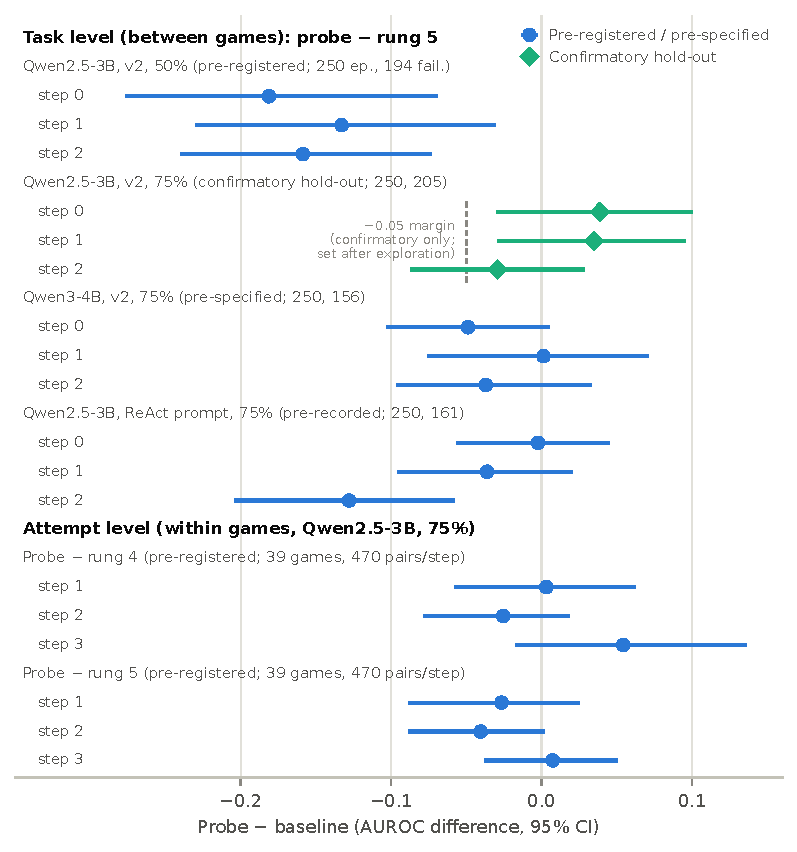
\includegraphics[width=0.82\linewidth]{fig3_probe_minus_baseline.pdf}
\caption{All pre-registered, pre-specified and confirmatory probe-versus-baseline comparisons (18; none superior). Points are AUROC differences with 95\% CIs. Task level: probe $-$ rung 5, scene-level cluster bootstrap (1,000 resamples); labels give the setting and $n$ (episodes, failures). Attempt level: within-game pairwise AUROC differences, game-level bootstrap (1,000 resamples); on label-shuffled data these intervals covered the null value only 80--94\% of the time (Section~\ref{sec:attempt}), so they are too narrow. Dashed segment: $-0.05$ non-inferiority margin, applied only to the confirmatory hold-out and set after the exploratory analysis. Exploratory estimates are not shown (Fig.~\ref{fig:heat}).}\label{fig:forest}
% Sources: results/probe_main_3b_primary_diff.csv, confirm_main_3b_diff.csv, task_qwen3_4b_diff_p.csv, task_react_qwen25_3b_diff_p.csv, within_game_diff.csv
\end{figure}


\subsection{Other actors and a second prompt}\label{sec:actors}
Of five further models piloted under a pre-registered inclusion rule, only Qwen3-4B passed (Appendix Tables~\ref{tab:a1}--\ref{tab:a2}). Its probe did not beat rung 5 in any round ($-0.049$, $+0.001$, $-0.037$; all inconclusive); its sampled rollouts rarely diverged (10 of 50 games with both outcomes), so its attempt-level question could not be answered (Appendix Table~\ref{tab:a3}).
Re-running Qwen2.5-3B with the original ReAct exemplars~\cite{yao2023react} (Appendix Table~\ref{tab:a4}) gave $-0.002$, $-0.036$ and $-0.128$ ($-0.204$ to $-0.058$): no round was superior and step 2 was inferior (Appendix Table~\ref{tab:settings}).
Across the four task-level evaluations the probe was superior to rung 5 in 0 of 12 rounds. A probe trained on v2 trajectories transferred poorly to ReAct trajectories (0.527, 0.493 and 0.555), which suggests that its direction is tied to the prompt format.

\subsection{Comparison with prior-style monitors}\label{sec:prior}
Approximating the task-blind baselines of earlier agent monitors (exploratory; Appendix Table~\ref{tab:prior}), the same probe beat a behavioral scorer after~\cite{ruan2026doomed} by $+0.145$ to $+0.190$ and a log-probability scorer after~\cite{pham2026agentstop} at steps 1 and 2.
Adding only the task type to the behavioral features raised its AUROC by 0.08--0.10, and against the full rung 5 the probe showed no advantage. A hidden-state advantage over task-blind monitors can thus disappear once the baseline sees the task.

\subsection{Early termination}
We evaluated stopping rules on the 500 greedy games with a 100-action horizon, measuring the mean largest fraction of steps saved at up to 10\% lost successes (Table~\ref{tab:early}). The probe saved 0.529 of the steps and a step cap 0.560; the primary difference was $-0.032$ ($-0.183$ to $+0.119$), inconclusive. This holds for the pre-specified range; over the whole loss range the probe saved more than the cap ($+0.056$) but less than rung 5t.
Secondary analyses suggest that where the probe helps over a fixed cap, a time-aligned surface baseline helps at least as much (rung 5t saved 0.625). Because 10\% of the successes is about 11 episodes, the intervals are wide.

% Generated by scripts/2026-10-21/extract_floats.py from paper/main_en.tex; edit the full manuscript, not this file.
\begin{table}[htbp]
\centering\small
\caption{Early termination, Qwen2.5-3B, 500 games, 100-action horizon.}\label{tab:early}
\begin{tabularx}{\linewidth}{@{}l>{\centering\arraybackslash}Xc@{}}
\toprule
Rule & Mean max.\ steps saved at $\le$10\% lost successes (95\% CI) & Relative to oracle \\
\midrule
Step cap & 0.560 (0.468, 0.656) & 0.58 \\
Loop detector & 0.194 (0.023, 0.361) & 0.20 \\
Rung 4t & 0.608 (0.477, 0.748) & 0.63 \\
Rung 5t & 0.625 (0.503, 0.758) & 0.65 \\
Probe (75\% depth + step) & 0.529 (0.382, 0.667) & 0.55 \\
Oracle (stop failures at step 0) & 0.958 (0.947, 0.969) & 1 \\
\bottomrule
\end{tabularx}
\end{table}


\subsection{Robustness}\label{sec:robust}
Relabeling with a 100-action horizon left no round superior. Five stronger probes (wider regularization, PCA, four depths concatenated, an MLP grid, and rung 5 with the hidden state added) gave none of 18 comparisons superior to rung 5, with the largest difference $+0.013$ (Appendix Table~\ref{tab:strength}).
Beyond the pre-registered rounds, differences at steps 0--10 ranged from $-0.114$ to $+0.009$, and probes on the running mean of hidden states were not better either. From step 7 on, rung 4 uses actions older than the six steps shown in the prompt.
Exploratory checks (first 250 episodes, plus one sweep on all 500; each run once): no narrowing of the probe minus rung 5 was detected as the training data grew, either on the first 250 episodes ($-0.002$ to $-0.025$ for about 50 to 200 training episodes) or on all 500 with fixed evaluation folds ($+0.016$ to $+0.006$ for about 50 to 400; change $-0.010$, 95\% CI $-0.038$ to $+0.022$, so a narrowing of up to about 0.02 is not ruled out; both methods were still improving); at a 10\% false-positive rate the probe detected 0.268 of failures and rung 5 0.407 (difference $-0.139$, $-0.273$ to $+0.075$); splitting by game changed the AUROC by $-0.006$ for the probe and $-0.027$ for rung 5; reading the hidden state at the last action token gave the same conclusion (75\% depth minus rung 5 $-0.019$, $-0.085$ to $+0.046$); and a sentence-encoder text baseline (bge-base-en-v1.5) was weaker than TF-IDF ($-0.115$). On shuffled labels, task-level intervals covered the null value in 85--90\% of runs rather than 95\% (the probe's 90\% cannot be told apart from 95\% or 80\%); widening the pre-registered intervals 1.26-fold kept all upper bounds below zero, step 1 only narrowly ($-0.004$).

\section{Discussion}
Across four task-level evaluations, a linear probe on the actor's hidden states was never better than a baseline built from visible information, and in the pre-registered cell it was worse.
Most of what any method predicted across games was the game itself; within games, failure was visible from step 2 on, but equally in the text and progress features.
Probes on agent hidden states have been reported to beat monitors that see only action-level features~\cite{ruan2026doomed}; our results suggest that such comparisons may overstate what hidden states add, since a ladder that sees the task closed the gap; we did not reproduce their environments, and our probe reads a different position, although reading the action token gave the same conclusion (Section~\ref{sec:robust}).
In math reasoning, an early probe fell to chance within problems~\cite{bulut2026problem}; our agent results differ in that within-game signals were above chance, likely because trajectories diverge in observable ways that both the text baseline and the probe can read (not tested).
Surface signals competing with internal ones has also been reported for web agents~\cite{pan2026monitoring}, and lightweight TF-IDF detectors found false success of agents better than LLM judges~\cite{advani2026false}; the weak transfer across prompts agrees with reports that truth-probe geometry depends on prompt templates~\cite{poulis2026truth}.

\paragraph{Why hidden states may not help here.} We see three explanations; only the third was examined directly, and only exploratorily. First, at the steps we evaluated the outcome is largely fixed by the game, and the prompt already states the task and the room, so the information the probe could use is also in the text.
Second, the probe may learn directions that encode the prompt's form rather than a general failure state, as the weak transfer across prompts suggests (the two prompts also differ in the token at which hidden states are taken).
Third, with about 200 training episodes per fold and 2,048 dimensions, a regularized linear probe may be too weak; however, 96 exploratory combinations of readers, depths and probe types, and five stronger probes, did not exceed the baseline either, and no change in the gap was detected between about 50 and 400 training episodes, nor between about 400 and 1,200 ($-0.008$; 95\% CI $-0.017$ to $+0.002$; 1,500 episodes). Reading five other positions of the prompt instead of the last template token gave AUROCs of 0.727--0.749 at 75\% depth, with no difference from the last prompt token or rung 5 resolved (post hoc).

\paragraph{A complementary reading.} Read at 75\% depth from a single token and trained on about 200 episodes per fold, the probe came within 0.011--0.034 AUROC of the engineered rung-5 baseline, and on the hold-out it was ahead at steps 0 and 1, though not significantly. Much of the failure-relevant information is linearly present in the representation; with the evaluation rows fixed, no change in the gap was detected between about 50 and 400 or between about 400 and 1,200 training episodes ($-0.008$; 95\% CI $-0.017$ to $+0.002$). The 75\% depth was chosen after seeing the exploratory depths; the pre-registered 50\% cell was 0.13--0.18 below rung 5.

\paragraph{Practical implication.} For small agents that run their own monitor, the hidden state costs nothing extra, so even a modest gain would be useful. We did not find one: at up to 10\% lost successes, a step cap saved about as many steps as the probe, and a surface baseline at least as many.
A simple cap or a monitor of the agent's text is a cheaper starting point and does not require access to model internals.

\paragraph{Methodological points.} Several design choices can change conclusions in similar studies. Splitting by game instead of by floor plan inflated a scene-only synthetic feature to an AUROC of 0.97 (with the real probe and rung 5 the change was small, $-0.006$ and $-0.027$).
Within-game evaluation was diluted by rollouts that had not yet diverged (52--70\% of pairs tied), and game-level percentile bootstrap intervals were too narrow on shuffled labels (coverage 80--94\% instead of 95\%; task level 85--90\%).
Whether attempts diverge at all depends on the policy: Qwen3-4B sampled at $T = 1$ diverged in only 10 of 50 games.

\section{Limitations}\label{sec:limits}
One environment, two Qwen models of 3--4B parameters and two prompts; three non-Qwen models solved only 1 of 20 pilot games under our prompt, which may reflect prompt--model fit. Actions were chosen by candidate scoring, not free generation.
With 250 episodes per evaluation set, intervals were about $\pm$0.06--0.10, so small differences cannot be resolved; the 75\% depth and the 0.05 margin were chosen after exploration; attempt-level results come from a sampling policy and from games selected by their greedy outcome; early-termination costs are counted in actions only; and the 7B reader was 4-bit quantized.
Pre-registered rounds cover only the first three actions. Episodes were cut at 30 actions; re-running the 399 greedy failures to 100 actions, 2.8\% succeeded late, and conclusions did not change with the 100-action label. The main prompt was written by us and adjusted on a different split before data collection; an external prompt was tested separately.
TF-IDF is a weak text baseline and the one neural encoder we tried was weaker still; low false-positive detection agreed with AUROC only in an exploratory check resting on 56 successes; task-level intervals covered the null in 85--90\% of shuffled-label runs rather than 95\%; the attainable AUROC from early states was not estimated; the 18 comparisons share games and baselines and are not independent; readers differ in hidden size (896 to 3,584 dimensions); and plans were registered as dated repository commits, not with an external registry (deviations in Appendix Table~\ref{tab:a8}). A second environment, a formal equivalence analysis and Monte Carlo value targets were not attempted, because they need new collection or a margin that was not registered. Training sets beyond about 1,200 episodes were not tried (the 1,000 extra episodes were a registered exception to the no-enlargement rule).

\section{Conclusion}
Linear probes on the hidden states of small Qwen agents did not predict ALFWorld failure better than a baseline built from the task, the prompt text and progress features, whether tested under a pre-registered plan, on a held-out set, with a second model or with an external prompt, and using them to stop doomed episodes was not shown to save more steps than a fixed limit at up to 10\% lost successes.
Claims that hidden states reveal agent failure should be tested against baselines that see the same task information, with evaluation within tasks.

\section*{Code and data availability}
Code, configurations, the analysis plans frozen before each run (with dates), the result tables behind the reported numbers and the figure scripts are in a public repository (link withheld for review). Collected trajectories and hidden states (3.6 GB) are not in the repository because of their size.
% To decide when the venue is chosen: the repository link (camera-ready) and how trajectories and hidden states are shared (e.g. a data DOI).

\bibliographystyle{unsrtnat}
\bibliography{refs}

\clearpage
\appendix
\section{Additional results and pre-registered items}
\setcounter{table}{0}\renewcommand{\thetable}{A\arabic{table}}
\setcounter{figure}{0}\renewcommand{\thefigure}{A\arabic{figure}}
The full version of this paper gives the complete method and all secondary analyses; the tables and figures below are identical to it.

% Generated by scripts/2026-10-21/extract_floats.py from paper/main_en.tex; edit the full manuscript, not this file.
\begin{table}[htbp]
\centering\small
\caption{Pre-registered hypothesis, decision rules and interpretation tables (wording from the frozen plans).}\label{tab:a7}
\begin{tabularx}{\linewidth}{@{}L>{\raggedright\arraybackslash}p{2.9cm}>{\raggedright\arraybackslash}p{2.9cm}@{}}
\toprule
Pre-registered item & Fixed & Observed \\
\midrule
\textbf{Task level.} H1: on 3B trajectories with the 3B reader, the probe AUROC at rounds 1--3 is higher than rung 5 (95\% CI of the difference excludes zero, above). & Before the primary run (2026-10-15) & Not supported: all three differences below zero \\
\addlinespace
Interpretation (a): only the 3B reader beats rung 5 $\rightarrow$ readable information has a size boundary. (b): all reader sizes beat it similarly $\rightarrow$ the information is at text level, so small models read it too. (c): even the 3B reader does not beat it $\rightarrow$ visible information suffices in this setting (negative result). & Before the primary run & (c) \\
\addlinespace
Decision rule for a difference: superior if the lower 95\% bound $> 0$; non-inferior if it $> -0.05$; inferior if the upper bound $< 0$; otherwise inconclusive. The 0.05 margin was set after the exploratory analysis. & Margin: after exploration, before the hold-out was evaluated & Hold-out: non-inferior, non-inferior, inconclusive (Table~\ref{tab:confirm}) \\
\addlinespace
\textbf{Attempt level.} Probe $>$ rungs 4 and 5 (lower 95\% bound $> 0$) $\rightarrow$ hidden states carry an in-progress failure signal not explained by difficulty text. Probe $\approx$ baseline $\rightarrow$ a signal exists but adds nothing beyond the history. All near 0.5 $\rightarrow$ success and failure within a game are not predicted by these methods. & Before the sampled rollouts were collected & Fits no row cleanly (Section~\ref{sec:attempt}) \\
\addlinespace
Supplementary rules for the attempt level: ``$\approx$'' only if the 95\% CI of the difference lies within $\pm 0.05$ (a lower bound above $-0.05$ alone is ``non-inferior, weak''); ``near 0.5'' if the CI includes 0.5 and the within-game permutation $p > 0.05$; Holm adjustment over the six comparisons. & Before the attempt-level results were opened (2026-10-17) & No comparison superior or equivalent \\
\bottomrule
\end{tabularx}
\par\smallskip\raggedright\footnotesize
% Sources: \code{docs/paper\_draft\_2026-10-15.md} (Section 2) and \code{docs/multi\_rollout\_plan\_2026-10-15.md} (interpretation rules, supplementary rules of 2026-10-17). The decision rule is also stated in Section~\ref{sec:stats}.
\end{table}

% Generated by scripts/2026-10-21/extract_floats.py from paper/main_en.tex; edit the full manuscript, not this file.
\begin{table}[htbp]
\centering\small
\caption{Deviations from the registered plans and exposures to results before a decision.}\label{tab:a8}
\footnotesize\setlength{\tabcolsep}{4pt}
\begin{tabularx}{\linewidth}{@{}>{\raggedright\arraybackslash}p{2.1cm}L>{\raggedright\arraybackslash}p{2.6cm}>{\raggedright\arraybackslash}p{2.8cm}@{}}
\toprule
Plan & Change or exposure & When & Effect on reported results \\
\midrule
Task-level freeze & Sample size raised from 250 to 500 episodes to create the confirmatory hold-out; policy, prompt and code unchanged & 2026-10-15, before the hold-out was collected & Hold-out analysed as one separate comparison \\
\addlinespace
Task-level freeze & Repository history rewritten to clean commit messages; the frozen commit hash changed (tree identical, mapping kept) & 2026-10-15 & None on data or code; registration rests on dated commits and the mapping \\
\addlinespace
Confirmatory comparison & Non-inferiority margin 0.05 chosen after the exploratory analysis & Before the hold-out was evaluated & Non-inferior labels are weak (Table~\ref{tab:confirm} note) \\
\addlinespace
Attempt level & Games stratified by greedy outcome, decided after the pilot & Before the main set was collected & Variance explained by the game is not a population value \\
\addlinespace
Attempt level & Supplementary analyses and interpretation rules added (equivalence band, near-0.5 rule, Holm adjustment) & 2026-10-17, before the results were opened & Primary verdicts reported unchanged; rules applied in addition \\
\addlinespace
Attempt level & Another session saw the first two lines of the results log (run size and the $\eta^2$ point estimate) & Before the attempt-level results were opened & Reported; no other result was seen \\
\addlinespace
100-action re-run & Interim counts seen twice during collection (3 late successes among the first 116 games); a partial collection was discarded after a shutdown & 2026-10-17, before the decision & Decision rule unchanged (committed beforehand) \\
\addlinespace
Early termination & Loop-detector definition clarified, then corrected so that the count excludes the action itself & 2026-10-20, before code was run and results opened & None on the other rules \\
\addlinespace
Model extension & Inclusion rule changed so that every model passing the pilot criteria enters & 2026-10-20, before the SmolLM3 pilot & Substitutes cannot be chosen after results; no further models added \\
\addlinespace
Model pilots & Reference time of the time criterion was not defined; judged against a reference value & 2026-10-17, after the first pilots & Exclusions rest on the success criterion \\
\addlinespace
Second prompt (ReAct) & Methods of the secondary success-rate comparison (Wilson CI, game-level bootstrap, exact McNemar) were not in the plan & 2026-10-20, fixed in the script before running & Secondary result only \\
\bottomrule
\end{tabularx}
\par\smallskip\raggedright\footnotesize
Compiled from the change logs of the plan documents; items already described in the text are repeated here so that all deviations appear in one place.
\end{table}

% Generated by scripts/2026-10-21/extract_floats.py from paper/main_en.tex; edit the full manuscript, not this file.
\begin{table}[htbp]
\centering\small
\caption{Confirmatory hold-out (episodes 250--499; 3B reader, 75\% depth, linear).}\label{tab:confirm}
\begin{tabularx}{\linewidth}{@{}Lccc@{}}
\toprule
 & Step 0 & Step 1 & Step 2 \\
\midrule
Probe AUROC (95\% CI) & 0.645 (0.547, 0.736) & 0.716 (0.619, 0.810) & 0.729 (0.633, 0.815) \\
Rung 5 AUROC & 0.607 & 0.681 & 0.758 \\
Probe $-$ rung 5 (95\% CI) & $+0.039$ ($-0.030$, $+0.100$) & $+0.035$ ($-0.030$, $+0.096$) & $-0.029$ ($-0.087$, $+0.029$) \\
Decision (margin 0.05, set post hoc) & non-inferior & non-inferior & inconclusive \\
\bottomrule
\end{tabularx}
\par\smallskip\raggedright\footnotesize
$n = 250$ episodes (205 failures). Training used all 500 episodes; evaluation used only the new 250. Margin sensitivity, read from the same intervals (lower bounds $-0.030$, $-0.030$, $-0.087$; upper bounds all above zero): with a margin of 0.025 no step would be non-inferior, and with 0.10 all three would be. Because the margin was set post hoc, the differences and intervals, not the labels, carry the evidence.
\end{table}

% Generated by scripts/2026-10-21/extract_floats.py from paper/main_en.tex; edit the full manuscript, not this file.
\begin{table}[htbp]
\centering\small
\caption{Task-level probe $-$ rung 5 (AUROC difference, 95\% CI) across settings.}\label{tab:settings}
\begin{tabularx}{\linewidth}{@{}Lccc@{}}
\toprule
Setting & Step 0 & Step 1 & Step 2 \\
\midrule
Qwen2.5-3B, v2, 50\% depth (pre-registered; $n = 250$, 194 failures) & $-0.181$ ($-0.276$, $-0.069$) & $-0.133$ ($-0.230$, $-0.031$) & $-0.159$ ($-0.240$, $-0.073$) \\
Qwen2.5-3B, v2, 75\% depth (confirmatory hold-out; 250, 205) & $+0.039$ ($-0.030$, $+0.100$) & $+0.035$ ($-0.030$, $+0.096$) & $-0.029$ ($-0.087$, $+0.029$) \\
Qwen3-4B, v2, 75\% depth (pre-specified; 250, 156) & $-0.049$ ($-0.103$, $+0.005$) & $+0.001$ ($-0.076$, $+0.071$) & $-0.037$ ($-0.096$, $+0.033$) \\
Qwen2.5-3B, ReAct prompt, 75\% depth (pre-recorded; 250, 161) & $-0.002$ ($-0.057$, $+0.045$) & $-0.036$ ($-0.096$, $+0.021$) & $-0.128$ ($-0.204$, $-0.058$) \\
\bottomrule
\end{tabularx}
\par\smallskip\raggedright\footnotesize
Probe and rung-5 AUROCs: Qwen3-4B 0.660/0.687/0.680 vs.\ 0.709/0.686/0.717; ReAct prompt 0.659/0.623/0.593 vs.\ 0.661/0.660/0.721. Scene-level cluster bootstrap, 1,000 resamples.
\end{table}

% Generated by scripts/2026-10-21/extract_floats.py from paper/main_en.tex; edit the full manuscript, not this file.
\begin{figure}[htbp]
\centering
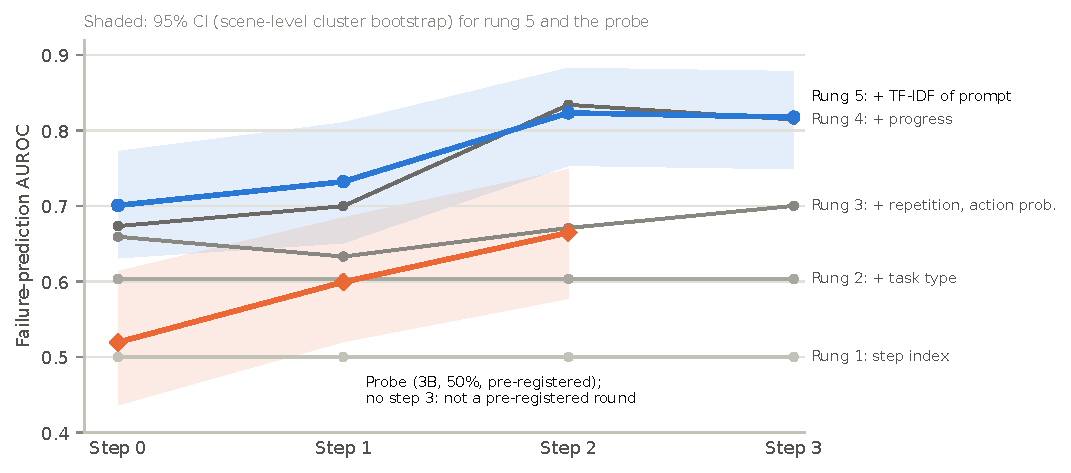
\includegraphics[width=\linewidth]{fig2_baseline_ladder.pdf}
\caption{Failure-prediction AUROC of the baseline ladder (steps 0--3) and the pre-registered probe (steps 0--2) on the first 250 episodes ($n = 250$, 194 failures per step). Rung 5 and the probe are emphasized, with shaded 95\% CIs from a scene-level cluster bootstrap (1,000 resamples); CIs of rungs 1--4 are omitted for legibility. Rung 1 is 0.5 by design and rung 2 does not change with the step. Overlap of the two shaded bands is not a test of their difference; the paired differences are in Fig.~\ref{fig:forest}.}\label{fig:ladder}
% Sources: results/baselines_main_3b.csv, results/probe_main_3b_primary.csv
\end{figure}

% Generated by scripts/2026-10-21/extract_floats.py from paper/main_en.tex; edit the full manuscript, not this file.
\begin{figure}[htbp]
\centering
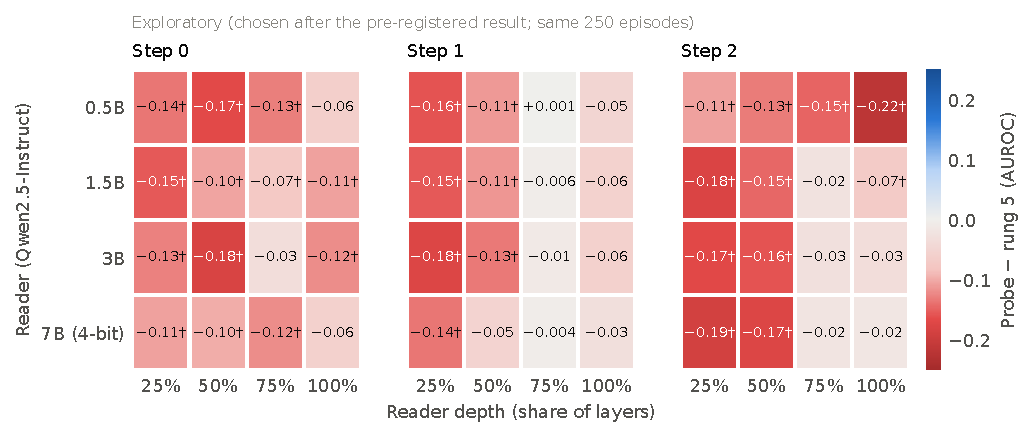
\includegraphics[width=\linewidth]{fig4_reader_depth.pdf}
\caption{Exploratory: probe $-$ rung 5 AUROC difference for every reader $\times$ depth of the linear probe on the first 250 episodes (48 cells, no selection). Diverging color centered on zero (red: probe below rung 5); $\dagger$ marks cells whose 95\% CI (scene-level cluster bootstrap) excludes zero, all of them below zero (31 of 48). No cell's CI lies above zero; the largest difference is $+0.001$. The 7B reader used 4-bit weights, so size is confounded with quantization. Linear and MLP cells with CIs: Appendix Table~\ref{tab:a9}.}\label{fig:heat}
% Source: results/explore_{0.5B,1.5B,3B,7B-4bit}_diff.csv
\end{figure}

% Generated by scripts/2026-10-21/extract_floats.py from paper/main_en.tex; edit the full manuscript, not this file.
\begin{table}[htbp]
\centering\small
\caption{Exploratory: linear-probe AUROC by reader and depth, first 250 episodes, mean over steps 0--2.}\label{tab:a6}
\begin{tabularx}{\linewidth}{@{}lccccL@{}}
\toprule
Reader & 25\% & 50\% & 75\% & 100\% & Probe $-$ rung 5, all 24 cells per reader (min, max) \\
\midrule
0.5B & 0.618 & 0.615 & \textbf{0.660} & 0.642 & $-0.277$, $+0.001$ \\
1.5B & 0.589 & 0.631 & \textbf{0.717} & 0.675 & $-0.195$, $-0.006$ \\
3B (= actor) & 0.595 & 0.594 & \textbf{0.727} & 0.682 & $-0.205$, $+0.004$ \\
7B (4-bit) & 0.608 & 0.643 & 0.704 & \textbf{0.717} & $-0.191$, $-0.004$ \\
\bottomrule
\end{tabularx}
\par\smallskip\raggedright\footnotesize
Rung 5 averaged 0.752 over steps 0--2. The last column covers both linear and MLP probes at all four depths and three steps (24 cells per reader, 96 in total). Best depth per reader in bold. The 3B reader at 50\% depth is the pre-registered cell (Table~\ref{tab:ladder}). Differences with 95\% CIs for all 96 cells are in Table~\ref{tab:a9}.
% Source: results/explore_{0.5B,1.5B,3B,7B-4bit}.csv and *_diff.csv
\end{table}

% Generated by scripts/2026-10-21/extract_floats.py from paper/main_en.tex; edit the full manuscript, not this file.
\begin{table}[htbp]
\centering\scriptsize
\setlength{\tabcolsep}{3pt}
\caption{Exploratory: probe $-$ rung 5 AUROC difference (95\% CI) for all 96 cells (4 readers $\times$ 2 probe types $\times$ 4 depths $\times$ 3 steps), first 250 episodes.}\label{tab:a9}
\begin{tabular}{@{}lllccc@{}}
\toprule
Reader & Probe & Depth & Step 0 & Step 1 & Step 2 \\
\midrule
0.5B reader & Linear & 25\% & $-0.136$ ($-0.236$, $-0.037$) & $-0.159$ ($-0.253$, $-0.061$) & $-0.106$ ($-0.191$, $-0.012$) \\
0.5B reader & Linear & 50\% & $-0.168$ ($-0.273$, $-0.065$) & $-0.112$ ($-0.223$, $-0.010$) & $-0.133$ ($-0.209$, $-0.049$) \\
0.5B reader & Linear & 75\% & $-0.130$ ($-0.212$, $-0.054$) & $+0.001$ ($-0.085$, 0.087) & $-0.148$ ($-0.229$, $-0.067$) \\
0.5B reader & Linear & 100\% & $-0.062$ ($-0.130$, 0.002) & $-0.050$ ($-0.125$, 0.029) & $-0.218$ ($-0.299$, $-0.131$) \\
0.5B reader & MLP & 25\% & $-0.259$ ($-0.386$, $-0.124$) & $-0.190$ ($-0.283$, $-0.078$) & $-0.277$ ($-0.373$, $-0.168$) \\
0.5B reader & MLP & 50\% & $-0.160$ ($-0.245$, $-0.083$) & $-0.160$ ($-0.272$, $-0.044$) & $-0.144$ ($-0.216$, $-0.063$) \\
0.5B reader & MLP & 75\% & $-0.163$ ($-0.242$, $-0.090$) & $-0.068$ ($-0.155$, 0.021) & $-0.154$ ($-0.232$, $-0.077$) \\
0.5B reader & MLP & 100\% & $-0.100$ ($-0.177$, $-0.025$) & $-0.012$ ($-0.096$, 0.075) & $-0.151$ ($-0.235$, $-0.071$) \\
1.5B reader & Linear & 25\% & $-0.155$ ($-0.231$, $-0.079$) & $-0.155$ ($-0.237$, $-0.075$) & $-0.179$ ($-0.274$, $-0.084$) \\
1.5B reader & Linear & 50\% & $-0.104$ ($-0.178$, $-0.032$) & $-0.113$ ($-0.201$, $-0.020$) & $-0.146$ ($-0.231$, $-0.066$) \\
1.5B reader & Linear & 75\% & $-0.074$ ($-0.154$, $-0.006$) & $-0.006$ ($-0.074$, 0.071) & $-0.025$ ($-0.097$, 0.047) \\
1.5B reader & Linear & 100\% & $-0.105$ ($-0.188$, $-0.024$) & $-0.055$ ($-0.129$, 0.023) & $-0.069$ ($-0.135$, $-0.004$) \\
1.5B reader & MLP & 25\% & $-0.173$ ($-0.261$, $-0.080$) & $-0.170$ ($-0.247$, $-0.094$) & $-0.161$ ($-0.241$, $-0.081$) \\
1.5B reader & MLP & 50\% & $-0.195$ ($-0.293$, $-0.086$) & $-0.074$ ($-0.163$, 0.017) & $-0.138$ ($-0.232$, $-0.058$) \\
1.5B reader & MLP & 75\% & $-0.167$ ($-0.240$, $-0.089$) & $-0.086$ ($-0.177$, 0.003) & $-0.069$ ($-0.135$, $-0.003$) \\
1.5B reader & MLP & 100\% & $-0.091$ ($-0.174$, $-0.007$) & $-0.097$ ($-0.185$, $-0.003$) & $-0.121$ ($-0.208$, $-0.035$) \\
3B reader (= actor) & Linear & 25\% & $-0.127$ ($-0.206$, $-0.061$) & $-0.176$ ($-0.269$, $-0.080$) & $-0.169$ ($-0.244$, $-0.087$) \\
3B reader (= actor) & Linear & 50\% & $-0.181$ ($-0.276$, $-0.069$) & $-0.133$ ($-0.230$, $-0.031$) & $-0.159$ ($-0.240$, $-0.073$) \\
3B reader (= actor) & Linear & 75\% & $-0.034$ ($-0.102$, 0.037) & $-0.011$ ($-0.082$, 0.061) & $-0.029$ ($-0.091$, 0.027) \\
3B reader (= actor) & Linear & 100\% & $-0.120$ ($-0.196$, $-0.056$) & $-0.057$ ($-0.147$, 0.032) & $-0.034$ ($-0.098$, 0.027) \\
3B reader (= actor) & MLP & 25\% & $-0.163$ ($-0.245$, $-0.075$) & $-0.153$ ($-0.259$, $-0.048$) & $-0.205$ ($-0.292$, $-0.105$) \\
3B reader (= actor) & MLP & 50\% & $-0.198$ ($-0.295$, $-0.106$) & $-0.189$ ($-0.290$, $-0.089$) & $-0.145$ ($-0.227$, $-0.063$) \\
3B reader (= actor) & MLP & 75\% & $+0.004$ ($-0.050$, 0.061) & 0.000 ($-0.069$, 0.069) & $-0.036$ ($-0.098$, 0.025) \\
3B reader (= actor) & MLP & 100\% & $-0.095$ ($-0.168$, $-0.025$) & $-0.057$ ($-0.145$, 0.031) & $-0.038$ ($-0.097$, 0.021) \\
7B reader (4-bit) & Linear & 25\% & $-0.107$ ($-0.208$, $-0.005$) & $-0.136$ ($-0.215$, $-0.051$) & $-0.189$ ($-0.277$, $-0.104$) \\
7B reader (4-bit) & Linear & 50\% & $-0.099$ ($-0.177$, $-0.019$) & $-0.053$ ($-0.141$, 0.032) & $-0.175$ ($-0.251$, $-0.097$) \\
7B reader (4-bit) & Linear & 75\% & $-0.119$ ($-0.189$, $-0.048$) & $-0.004$ ($-0.094$, 0.093) & $-0.021$ ($-0.080$, 0.046) \\
7B reader (4-bit) & Linear & 100\% & $-0.058$ ($-0.141$, 0.022) & $-0.030$ ($-0.113$, 0.056) & $-0.017$ ($-0.080$, 0.050) \\
7B reader (4-bit) & MLP & 25\% & $-0.154$ ($-0.251$, $-0.051$) & $-0.132$ ($-0.232$, $-0.028$) & $-0.144$ ($-0.229$, $-0.060$) \\
7B reader (4-bit) & MLP & 50\% & $-0.191$ ($-0.286$, $-0.096$) & $-0.122$ ($-0.221$, $-0.021$) & $-0.149$ ($-0.226$, $-0.072$) \\
7B reader (4-bit) & MLP & 75\% & $-0.124$ ($-0.216$, $-0.036$) & $-0.079$ ($-0.162$, 0.011) & $-0.094$ ($-0.170$, $-0.020$) \\
7B reader (4-bit) & MLP & 100\% & $-0.071$ ($-0.158$, 0.012) & $-0.087$ ($-0.177$, 0.001) & $-0.039$ ($-0.115$, 0.031) \\
\bottomrule
\end{tabular}
\par\smallskip\raggedright\footnotesize
Scene-level cluster bootstrap, 1,000 resamples; $n = 250$ (194 failures) per step. The 7B reader used 4-bit weights. The 3B reader at 50\% depth (linear) is the pre-registered cell.
% Source: results/explore_{0.5B,1.5B,3B,7B-4bit}_diff.csv
\end{table}

% Generated by scripts/2026-10-21/extract_floats.py from paper/main_en.tex; edit the full manuscript, not this file.
\begin{table}[htbp]
\centering\small
\caption{Exploratory: task-level AUROC of prior-style baselines, first 250 episodes.}\label{tab:prior}
\begin{tabularx}{\linewidth}{@{}Lccc@{}}
\toprule
 & Step 0 & Step 1 & Step 2 \\
\midrule
Behavioral features (after~\cite{ruan2026doomed}) & 0.522 & 0.554 & 0.605 \\
Log-probability features (after~\cite{pham2026agentstop}) & 0.626 & 0.545 & 0.606 \\
Behavioral + task type & 0.626 & 0.656 & 0.689 \\
Rung 5 & 0.701 & 0.732 & 0.823 \\
Probe (75\% depth, linear) & 0.666 & 0.721 & 0.795 \\
\addlinespace
Probe $-$ behavioral (95\% CI) & $+0.145$ (0.032, 0.247) & $+0.167$ (0.070, 0.247) & $+0.190$ (0.107, 0.282) \\
Probe $-$ log-probability (95\% CI) & $+0.040$ ($-0.060$, 0.133) & $+0.176$ (0.051, 0.297) & $+0.189$ (0.074, 0.296) \\
Probe $-$ rung 5 (95\% CI) & $-0.034$ ($-0.102$, 0.037) & $-0.011$ ($-0.082$, 0.061) & $-0.029$ ($-0.091$, 0.027) \\
\bottomrule
\end{tabularx}
\par\smallskip\raggedright\footnotesize
$n = 250$ (194 failures) per step; scene-level cluster bootstrap, 1,000 resamples.
% Source: results/prior_methods_3b*.csv
\end{table}

% Generated by scripts/2026-10-21/extract_floats.py from paper/main_en.tex; edit the full manuscript, not this file.
\begin{table}[htbp]
\centering\small
\caption{Exploratory: stronger probes $-$ rung 5 (AUROC difference, 95\% CI), first 250 episodes.}\label{tab:strength}
\begin{tabularx}{\linewidth}{@{}Lccc@{}}
\toprule
Probe & Step 0 & Step 1 & Step 2 \\
\midrule
Reference (75\% depth, linear, $C \le 1$) & $-0.034$ ($-0.102$, 0.037) & $-0.011$ ($-0.082$, 0.061) & $-0.029$ ($-0.091$, 0.027) \\
Wider $C$ grid & $-0.036$ ($-0.105$, 0.036) & $+0.013$ ($-0.072$, 0.101) & $-0.034$ ($-0.099$, 0.026) \\
PCA ($k$ 8--128) & $-0.019$ ($-0.084$, 0.041) & $-0.037$ ($-0.103$, 0.032) & $-0.029$ ($-0.091$, 0.026) \\
Four depths concatenated & $-0.052$ ($-0.121$, 0.008) & $-0.055$ ($-0.127$, 0.023) & $-0.077$ ($-0.159$, $-0.003$) \\
MLP (grid of 4) & $-0.036$ ($-0.104$, 0.023) & $-0.025$ ($-0.105$, 0.058) & $-0.052$ ($-0.122$, 0.017) \\
Rung 5 + hidden state & $-0.034$ ($-0.101$, 0.037) & $-0.023$ ($-0.096$, 0.047) & $-0.024$ ($-0.086$, 0.032) \\
\bottomrule
\end{tabularx}
\par\smallskip\raggedright\footnotesize
Rung 5 AUROC 0.701, 0.732, 0.823. $n = 250$ (194 failures) per step; scene-level cluster bootstrap, 1,000 resamples.
% Sources: results/probe_strength_3b*.csv, results/extra_main_3b_B_late_rounds.csv, results/extra_main_3b_C_temporal.csv
\end{table}

% Generated by scripts/2026-10-21/extract_floats.py from paper/main_en.tex; edit the full manuscript, not this file.
\begin{table}[htbp]
\centering\small
\caption{Model pilots (first 20 games, v2 prompt, candidate scoring, 30 actions).}\label{tab:a1}
\footnotesize\setlength{\tabcolsep}{4pt}
\begin{tabularx}{\linewidth}{@{}L>{\centering\arraybackslash}p{2.2cm}c>{\centering\arraybackslash}p{1.6cm}>{\raggedright\arraybackslash}p{2.6cm}@{}}
\toprule
Model & Successes (Wilson 95\% CI) & s / episode & Peak GPU memory & Decision \\
\midrule
Qwen3-4B (thinking off) & 7/20 (18--57\%) & 14.9 & 10.24\,GB & included \\
Qwen3-1.7B (thinking off) & 1/20 (1--24\%) & 8.5 & 5.03\,GB & excluded (successes) \\
Llama-3.2-3B-Instruct & 1/20 (1--24\%) & 10.7 & 8.06\,GB & excluded (successes) \\
SmolLM3-3B & 1/20 (1--24\%) & 10.4 & 7.41\,GB & excluded (successes) \\
Phi-3.5-mini-instruct (candidates scored in batches of 4) & 1/20 (1--24\%) & 67.6 & 10.75\,GB & excluded (successes, time) \\
\bottomrule
\end{tabularx}
\par\smallskip\raggedright\footnotesize
Reference on the same games: Qwen2.5-3B 5/20. All runs completed, all actions were admissible and no hidden state was non-finite. Revisions were pinned; chat-template dates were fixed (Llama ``26 Jul 2024'', SmolLM3 ``20 October 2026'').
\end{table}

% Generated by scripts/2026-10-21/extract_floats.py from paper/main_en.tex; edit the full manuscript, not this file.
\begin{table}[htbp]
\centering\small
\caption{Exploratory: action patterns on the 20 pilot games.}\label{tab:a2}
\footnotesize\setlength{\tabcolsep}{4pt}
\begin{tabularx}{\linewidth}{@{}lc>{\centering\arraybackslash}p{2.2cm}>{\centering\arraybackslash}p{1.8cm}L@{}}
\toprule
Model & Successes & Repeated within last 6 steps & Distinct-action ratio & Most frequent verbs \\
\midrule
Qwen2.5-3B & 5/20 & 51\% & 0.44 & go 67\%, take 11\%, move 8\% \\
Qwen3-4B & 7/20 & 32\% & 0.54 & go 60\%, examine 14\%, open 9\% \\
Llama-3.2-3B & 1/20 & 66\% & 0.26 & examine 47\%, go 28\%, open 12\% \\
SmolLM3-3B & 1/20 & 82\% & 0.19 & examine 57\%, take 15\%, move 14\% \\
Phi-3.5-mini & 1/20 & 76\% & 0.25 & take 33\%, move 30\%, go 16\% \\
\bottomrule
\end{tabularx}
\end{table}

% Generated by scripts/2026-10-21/extract_floats.py from paper/main_en.tex; edit the full manuscript, not this file.
\begin{table}[htbp]
\centering\small
\caption{Qwen3-4B within-game pairwise AUROC ($T = 1$ sampling; 10 of 50 games with both outcomes, 120 pairs per step).}\label{tab:a3}
\begin{tabularx}{\linewidth}{@{}Lccc@{}}
\toprule
 & Step 1 & Step 2 & Step 3 \\
\midrule
Probe (own hidden state, 75\% depth, linear) & 0.471 (0.396, 0.500) & 0.471 (0.397, 0.509) & 0.479 (0.402, 0.517) \\
Rung 4 & 0.479 (0.404, 0.519) & 0.471 (0.397, 0.509) & 0.521 (0.443, 0.611) \\
Rung 5 & 0.471 (0.391, 0.508) & 0.471 (0.397, 0.509) & 0.521 (0.443, 0.611) \\
Probe $-$ rung 4 (95\% CI) & $-0.008$ ($-0.020$, 0.000) & 0.000 (0.000, 0.000) & $-0.042$ ($-0.202$, $+0.063$) \\
Probe $-$ rung 5 (95\% CI) & 0.000 ($-0.011$, $+0.015$) & 0.000 (0.000, 0.000) & $-0.042$ ($-0.202$, $+0.063$) \\
Within-game permutation $p$, probe & 1.00 & 0.94 & 0.92 \\
\bottomrule
\end{tabularx}
\par\smallskip\raggedright\footnotesize
Game-level bootstrap (1,000 resamples). $\eta^2 = 0.849$ (0.747--0.935); difficulty oracle alone 0.911 on pooled rows. Most pairs were tied (identical prompts), so these values carry little information; by a decision made before the results were read, no conclusion is drawn (Section~\ref{sec:actors}).
% Source: results/within_game_qwen3_4b*.csv
\end{table}

% Generated by scripts/2026-10-21/extract_floats.py from paper/main_en.tex; edit the full manuscript, not this file.
\begin{table}[htbp]
\centering\small
\caption{The two prompts.}\label{tab:a4}
\begin{tabularx}{\linewidth}{@{}lLL@{}}
\toprule
 & v2 (ours) & ReAct exemplars (minimally edited) \\
\midrule
Source & Written by us; earlier version in ReAct thought--action format; frozen before data collection & Yao et al.\ (2023), \code{alfworld\_3prompts.json}, repository commit \code{6bdb3a1} \\
Format & Chat template (system + user message) & Raw completion text ending in \code{>} \\
Instructions & Six rules & One header line \\
Exemplars & One handwritten episode (clean task), same for all tasks & Two original episodes matched to the current task type, including \code{think:} lines \\
History & Last six steps & Full episode \\
Admissible actions in prompt & Yes, plus recently failed actions & No (scoring still restricted to admissible actions) \\
Scored continuation & \code{Action: a<|im\_end|>} & \code{\textvisiblespace a\textbackslash n} \\
Hidden-state token & Last token of the generation prompt & Final \code{>} \\
Edits & -- & \code{put A in/on B} $\rightarrow$ \code{move A to B} and the matching observation \\
Length (Qwen2.5 tokens) & median 864 (whole prompt) & 1,115--1,571 (exemplars only) \\
\bottomrule
\end{tabularx}
\end{table}

% Generated by scripts/2026-10-21/extract_floats.py from paper/main_en.tex; edit the full manuscript, not this file.
\begin{table}[htbp]
\centering\small
\caption{Preliminary runs before the policy was fixed (2026-10-08).}\label{tab:a5}
\begin{tabularx}{\linewidth}{@{}Lccc@{}}
\toprule
Run & Episodes & Successes & Admissible actions \\
\midrule
Free generation, first prompt (Thought/Action), 0.5B & 2 & 0 & 8\% \\
Free generation, first prompt, 1.5B & 5 & 0 & 56\% \\
Free generation, first prompt, 3B & 5 & 1 & 61\% \\
Free generation, 1.5B, first code on the GPU machine & 3 & 0 & 26\% \\
Free generation, 1.5B, revised prompt (rules and example) & 5 & 0 & 22\% \\
Candidate scoring (final policy), 0.5B / 1.5B / 3B, training games & 20 / 100 / 100 & 0 / 2 / 20 & 100\% by construction \\
\bottomrule
\end{tabularx}
\par\smallskip\raggedright\footnotesize
Free-generation runs used Qwen2.5-Instruct models on ALFWorld training games before the prompt was frozen; with so few episodes they only show that inadmissible actions were frequent. Source: project log of 2026-10-08; the raw run logs were not kept in the repository or its backups.
\end{table}


\end{document}
